\documentclass[11pt]{article}
\usepackage{latexsym}
\usepackage{amsmath}
\usepackage{amssymb}
\usepackage{amsthm}
\usepackage{epsfig}
\usepackage{algpseudocode}
\usepackage{float} 
\usepackage[tight]{subfigure}

\usepackage{amsmath}
\usepackage{hyperref}

\DeclareMathOperator*{\minimize}{min}
\DeclareMathOperator*{\maximize}{max}

\usepackage{algorithm}
 %on linux you may need to run sudo apt-get install texlive-full to install algorithm.sys
% \usepackage{algorithmic}

\usepackage{verbatim}

\newcommand{\handout}[5]{
  \noindent
  \begin{center}
  \framebox{
    \vbox{
      \hbox to 5.78in { {#1} \hfill #2 }
      \vspace{4mm}
      \hbox to 5.78in { {\Large \hfill #5  \hfill} }
      \vspace{2mm}
      \hbox to 5.78in { {\em #3 \hfill #4} }
    }
  }
  \end{center}
  \vspace*{4mm}
}

\newcommand{\lecture}[5]{\handout{#1}{#2}{#3}{#4}{#5}}
\newcommand{\collision}[0]{\mathrm{collision}}
\newcommand{\nocollision}[0]{\overline{\collision}}

\newcommand*{\QED}{\hfill\ensuremath{\square}}

\newtheorem{theorem}{Theorem}
\newtheorem{corollary}[theorem]{Corollary}
\newtheorem{lemma}[theorem]{Lemma}
\newtheorem{observation}[theorem]{Observation}
\newtheorem{proposition}[theorem]{Proposition}
\newtheorem{definition}[theorem]{Definition}
\newtheorem{claim}[theorem]{Claim}
\newtheorem{fact}[theorem]{Fact}
\newtheorem{assumption}[theorem]{Assumption}
\newtheorem{note}[theorem]{Note}

% 1-inch margins, from fullpage.sty by H.Partl, Version 2, Dec. 15, 1988.
\topmargin 0pt
\advance \topmargin by -\headheight
\advance \topmargin by -\headsep
\textheight 8.9in
\oddsidemargin 0pt
\evensidemargin \oddsidemargin
\marginparwidth 0.5in
\textwidth 6.5in

\parindent 0in
\parskip 1.5ex
%\renewcommand{\baselinestretch}{1.25}

\begin{document}

\lecture{Statistical Techniques in Robotics (16-831, S22)}{Lecture \#14
  (Monday, March 14)}{Lecturer: Kris Kitani}{Scribes: Yimin Tang, Zilin Si}{RL \& MDP}

\section{Review}
In the last lecture, we learnt the Thompson Sampling in the Stochastic environment, EXP3 and EXP4 in the adversarial environment which is context-free and contextual respectively.

\subsection{Thompsons Sampling: Beta-Bernoulli Bandit}
We use beta-bernoulli distribution to estimate the each arm's reward function since these two are conjugate. Therefore the algorithm is shown as below:
\begin{algorithm}
\caption{Bern-Beta Thompsons Sampling}
\begin{algorithmic}[1]
    \For{$t=1...T$}
        \State $\theta_t \sim p(\theta; \alpha_k, \beta_k), \forall k$ \hfill $\triangleright$ sample from posterior
        \State $a^{(t)}_{\hat{k}} = argmax_{k} \mathbb{E}_{p(r|a_k, \theta_k)} [r|a_k, \theta_k]$ \hfill $\triangleright$ predict
        \State $REVEIVE(r^{(t)})$ \hfill $\triangleright$ get reward
        \State $\alpha_{\hat{k}} = \alpha_{\hat{k}} + r^{(t)}$ 
        \State $\beta_{\hat{k}} = \beta_{\hat{k}} + 1 - r^{(t)}$ \hfill $\triangleright$ update posterior
    \EndFor
\end{algorithmic}
\end{algorithm}

The regret of Thompson Sampling is $O(\sqrt{KT logT})$

\subsection{EXP3}
EXP3 stands for ``exponential-weight update algorithm for exploration and exploitation".

\begin{algorithm}
\caption{EXP3($\gamma \in [0,1]$)}
\begin{algorithmic}[1]

\State $\mathbf{\omega}^{(1)} \leftarrow \{ \omega_k^{(1)} = 1\}_{k=1}^{K}$ \hfill $\triangleright$ wights over actions
    \For{$t=1...T$}
        \State $p^{(t)} = \frac{\omega^{(t)}}{\sum_{k}\omega_{k}^{(t)}}$ \hfill $\triangleright$ probability over actions
        \State $k \sim MULTINOMIAL(p^{(t)})$
        \State $a^{(t)} = a_k$ \hfill $\triangleright$ take and draw action
        \State $REVEIVE(r^{(t)} \in [0,1])$ \hfill $\triangleright$ get reward
        \State $\omega_{k}^{(t+1)} = \omega_{k}^{(t)} exp\{\gamma \cdot r^{(t)} / p_k^{(t)}\}$ \hfill $\triangleright$ update weight for one arm
    \EndFor
\end{algorithmic}
\end{algorithm}

where the update term $r^{(t)}/p_k^{(t)}$ is the unbiased estimator.

The regret of EXP3 is $O(\sqrt{TK log K})$ and it is a no regret algorithm.

\subsection{EXP4}
EXP4 stands for ``exponential-weight update algorithm for exploration and exploitation with experts".

\begin{algorithm}
\caption{EXP4($\gamma \in [0,1], T$)}
\begin{algorithmic}[1]

\State $\mathbf{\omega}^{(1)} \leftarrow \{ \omega_k^{(1)} = 1\}_{k=1}^{K}$ \hfill $\triangleright$ wights over experts
    \For{$t=1...T$}
        \State $RECEIVE(X^{(t)} \in \mathbb{R}^{N \times K})$ \hfill $\triangleright$ advice from N experts
        \State $q^{(t)} = \frac{\omega^{(t)}}{||\omega^{(t)}||} \cdot X^{(t)} \in \Delta^K$ \hfill $\triangleright$ probability over actions
        \State $k^{(t)} \sim MULTINOMIAL(q^{(t)})$ \hfill $\triangleright$ draw action
        \State $RECEIVE(r^{(t)})$ \hfill $\triangleright$ get reward
        \State $\hat{r}^{(t)} = \frac{r^{(t)}}{q_{k}^{(t)}} \mathbb{I}[k = k^{(t)}] \in \mathbb{I}^K$ \hfill $\triangleright$ reward over all arms
        \State $g^{(t)} = X^{(t)} \cdot \hat{r}^{(t)} \in \mathbb{R}^N$ \hfill $\triangleright$ per expert reward
        \State $\omega_{n}^{(t+1)} = \omega_{n}^{(t)} exp\{\gamma \cdot g_n^{(t)}\} \forall n$ \hfill $\triangleright$ update weight for all arms
    \EndFor
\end{algorithmic}
\end{algorithm}

The regret of EXP4 is $O(\sqrt{TK log N})$ where $K$ is the number of arms, $T$ is the time, and $N$ is the number of experts.

\section{Summary}

\subsection{Sequence Feedback Learning Problems}
To distinguish the sequence feedback or one-shot feedback, a good indicator would be whether the data generation (feedback) a sequentially dependent process.
\paragraph{One-Shot Feedback}
Supervised learning is one kind of one-shot feedback. If we draw samples from the data distribution as 
\begin{equation}
    x, a \sim \mathit{D} (x, a)
\end{equation}
here we assume $x$ is the state and $a$ is the action. then we can get a set of identically and independently distributed (i.i.d) samples as $\{(x_1, a_1), (x_2, a_2), ..., (x_N, a_N)\}$. This means the action from the previous sample $a_{i-1}$ won't affect the state in the next sample $x_{i}$. For one-shot feedback, we don't need to worry about issues like co-variate shift or temporal credit assignment.
\paragraph{Sequence Feedback}
Reinforcement learning is one kind of sequence feedback. If we draw samples from the data distribution as 
\begin{equation}
    \zeta, R \sim \mathit{D} (\zeta, R)
\end{equation}
where $\zeta = \{(x_1, a_1), (x_2, a_2), ..., (x_N, a_N)\}$ is a trajectory of samples where all samples are correlated, $R_i \in \mathbb{R}$ is the reward for the entire sequence. Under this circumstance, the action affects the next state and we need to address covariate shift, temporal credit assignment, very large "trajectory" space.

\subsection{Review of Learning Problems}
As shown in the Table~\ref{table:decision_making}, we classified the decision-making problems covered so far into sampled/exhausted, evaluative/instructive, sequential/one-shot. 
Note that:\\
1) For PWEA, the loss function is fully observed so all parameters could be updated at every step. So it is instructive. \\
2) For MAB, C-MAB, the reward function is only partial observed so we could only update one (arm) parameter at a time. So it is evaluative.\\
3) For all problems including PWEA, OLC/OMD, MAB, C-MAB, their feedback is one-shot. \\
4) For sequential problem such as RL, we have to reason about the impact of decisions on the entire sequence including the future. So we obtain a sequence of rewards, update the future predictor (value function), and then update the action predictor (policy).
\begin{table}[]
3\centering
\begin{tabular}{|l|l|l|l|}
\hline
Problem & Sampled & Evaluative & Sequential \\ \hline
PWEA    &    $\times$     &      $\times$      &    $\times$        \\ \hline
OLC/OMD &    $\surd$     &      $\triangle$      &     $\times$       \\ \hline
MAB     &    $\times$     &      $\surd$       &     $\times$       \\ \hline
C-MAB   &    $\surd$     &       $\surd$      &      $\times$      \\ \hline
RL      &    $\surd$     &       $\surd$      &     $\surd$        \\ \hline
IL      &     $\surd$    &      $\surd$       &    $\triangle$        \\ \hline
\end{tabular}
\caption{Table for decision-making problems classification.}
\label{table:decision_making}
\end{table}

\subsection{Markov Decision Process}
\begin{figure}[htbp]
    \centering
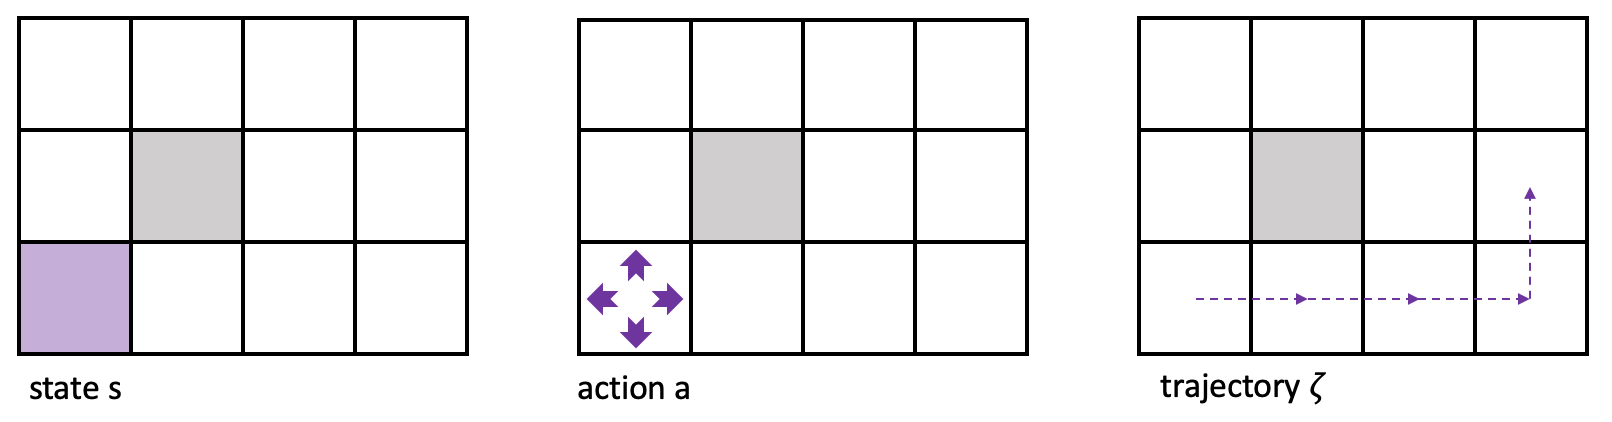
\includegraphics[width=15cm]{imgs/Grid_World.png}
    \caption{State $s$, action $a$, and trajectory $\zeta$ defined in a grid world.}
    \label{fig:grid}
\end{figure} 

First we use a grid world as example to define the components of markov decision process (MDP) as shown in Fig.~\ref{fig:grid}. Each grid is one state $s$. Each movement is one action $a$ including moving up, moving down, moving left and moving right. A trajectory is a sequence of states and actions as $\zeta = \{ s_0, a_0, s_1, a_1, ..., s_T, a_T\}$. 


Here we consider the joint distribution
\begin{equation}
    p(s_0, a_0, s_1, a_1, ..., s_T, a_T)
\end{equation}
 as the probability of a state-action trajectory. We can factorize it as
\begin{equation}
    p(s_0, a_0, s_1, a_1, ..., s_T, a_T) = p_0(s_0) \prod_{t} p(s_{t+1}| s_t, a_t) p(a_t|s_t)
\end{equation}
where $p_0(s_0)$ is the prior state. $p(s_{t+1}| s_t, a_t)$ is the state transition dynamic which describe the probability of transition to another state. $p(a_t|s_t)$ is the policy which describes which action to take in a given state which can be stochastic or deterministic. 
 
 And a reward function 
\begin{equation}
    r(s_0, a_0, s_1, a_1, ..., s_T, a_T)
\end{equation}
as a scalar value for one trajectory. We can factorize it as 
\begin{equation}
\begin{split}
    r(s_0, a_0, s_1, a_1, ..., s_T, a_T) & = r(s_0, a_0, s_1) + r(s_1, a_1, s_2) + ... \\
    & \Leftrightarrow r(s_0, a_0) + r(s_1, a_1) + ... \\
    & \Leftrightarrow r(s_0) + r(s_1) + ... 
\end{split}
\end{equation}
where $r(s)$ maps a state to a real value.

We can model the markov decision process as a graphical model as shown in Fig.~\ref{fig:graph}.

\begin{figure}[htbp]
    \centering
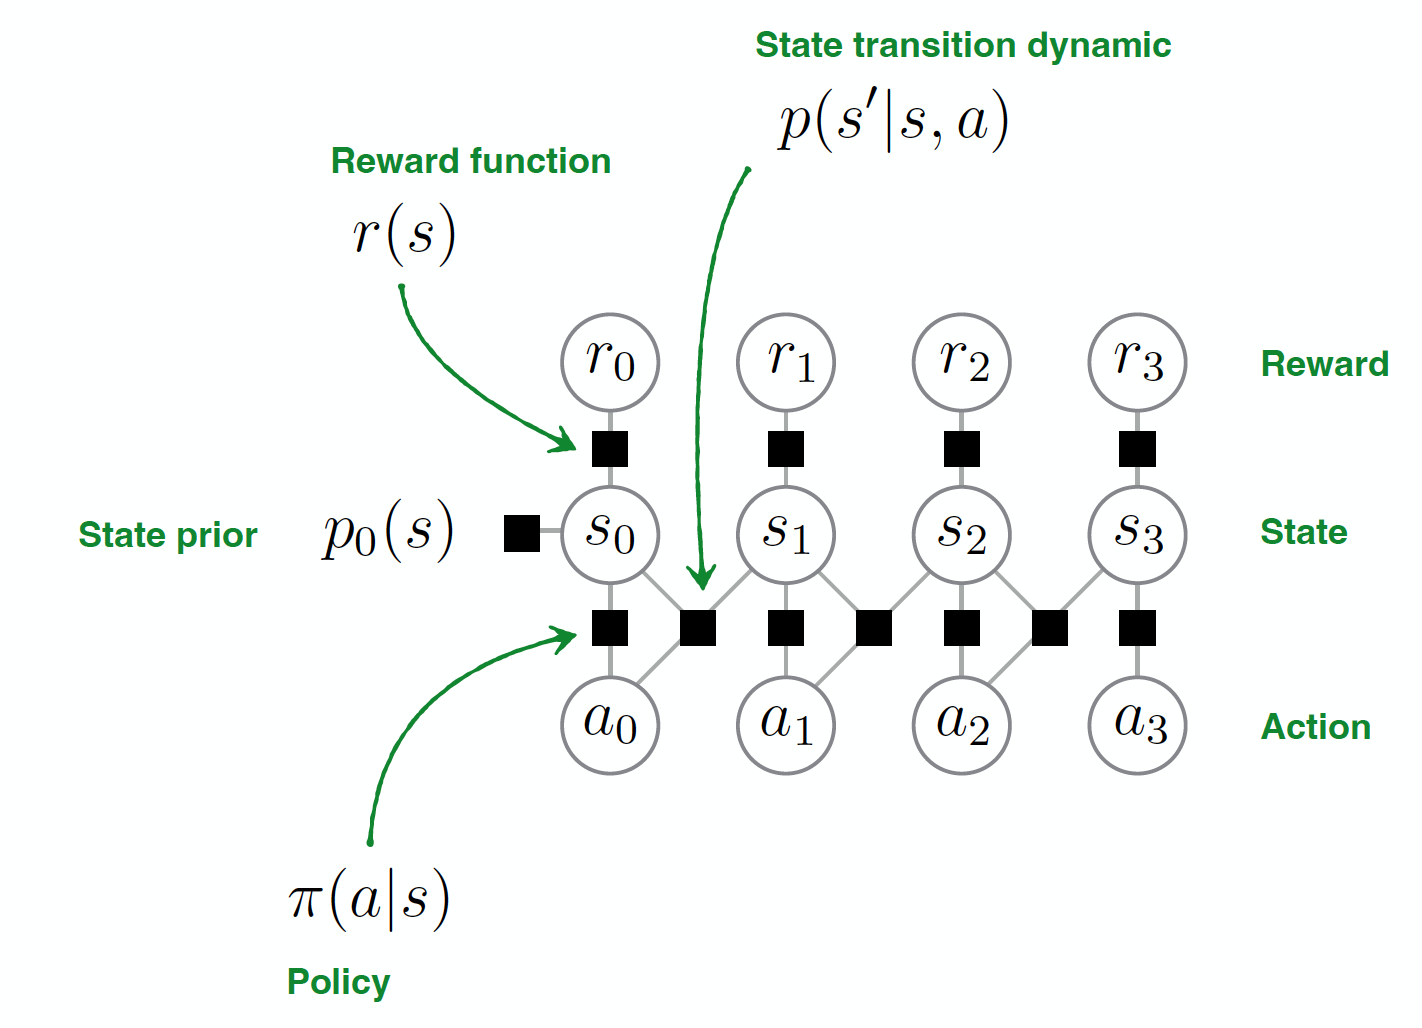
\includegraphics[width=15cm]{imgs/graph_model.png}
    \caption{Graphical model for markov decision process.}
    \label{fig:graph}
\end{figure} 

\subsection{Mathematic of the MDP}

\subsubsection{Value Function}

We can define a value function for one policy on states:

\begin{equation}
V^{\pi}(s)=\mathbb{E}_{p}\left[r_{0}+r_{1}+r_{2}+\cdots \mid s_{0}=s\right]
\end{equation}

$\pi$ is our policy, $r_{0}, r_{1}, r_{2}, \cdots$ is all rewards for one trajectory generated by our policy and the environment when start state is $s$, and $p$ is the trajectory probability which can be writen by:

\begin{equation}
p\left(s_{0}, a_{0}, s_{1}, a_{1}, \cdots\right)=p_{0}\left(s_{0}\right) p\left(s_{1} \mid s_{0}, a_{0}\right) p\left(a_{0} \mid s_{0}\right) p\left(s_{2} \mid s_{1}, a_{1}\right) p\left(a_{1} \mid s_{1}\right) \cdots
\end{equation}

Notice $r_{0}, r_{1}, r_{2}, \cdots$, we can choose different time horizons:
\begin{itemize}
\item  \textbf{Infinite horizon return}: $V^{\pi}(s)=\mathbb{E}_{p}\left[r_{0}+r_{1}+r_{2}+\cdots \mid s_{0}=s\right]$
\item  \textbf{Finite horizon return}: $V^{\pi}(s)=\mathbb{E}_{p}\left[r_{0}+r_{1}+r_{2}+\cdots+r_{T} \mid s_{0}=s\right]$
\item  \textbf{Infinite horizon discounted return}: $V^{\pi}(s)=\mathbb{E}_{p}\left[\gamma^{0} r_{0}+\gamma^{1} r_{1}+\gamma^{2} r_{2}+\cdots \mid s_{0}=s\right]$

\end{itemize}


We can also define state-action value function based on our policy in infinite horizon discounted return form:

\begin{equation}
Q^{\pi}(s, a)=\mathbb{E}_{p}\left[\gamma^{0} r\left(s_{0}\right)+\gamma^{1} r\left(s_{1}\right)+\gamma^{2} r\left(s_{2}\right)+\cdots \mid s_{0}=s, a_{0}=a\right] 
\end{equation}

Consider $Q^{\pi}(s, a)$ and $V^{\pi}(s)$, we can get:

\begin{align*}
V^{\pi}(s) &=\mathbb{E}\left[\sum_{t=0}^{\infty} \gamma^{t} r_{t} \mid s_{0}=s\right] \\
&=\sum_{s_{1: \infty}, a_{0: \infty}} p\left(s_{1: \infty}, a_{0: \infty}\right)\left[\sum_{t=0}^{\infty} \gamma^{t} r_{t} \mid s_{0}=s\right] \\
&=\sum_{s_{1: \infty}, a_{0}: \infty} \pi\left(a_{0} \mid s_{0}=s\right) p\left(s_{1: \infty}, a_{1: \infty}\right)\left[\sum_{t=0}^{\infty} \gamma^{t} r_{t} \mid s_{0}=s\right] \\
&=\sum_{a} \pi\left(a_{0}=a \mid s_{0}=s\right) \sum_{s_{1: \infty}, a_{1: \infty}} p\left(s_{1: \infty}, a_{1: \infty}\right)\left[\sum_{t=0}^{\infty} \gamma^{t} r_{t} \mid s_{0}=s, a_{0}=a\right] \\
&=\sum_{a} \pi\left(a_{0}=a \mid s_{0}=s\right) \mathbb{E}\left[\sum_{t=0}^{\infty} \gamma^{t} r_{t} \mid s_{0}=s, a_{0}=a\right] \\
&=\sum_{a} \pi(a \mid s) Q^{\pi}(s, a) \quad
\end{align*}



\subsubsection{Bellman Equation}

We can change:
\begin{align*}
V^{\pi}(s) =\sum_{a} \pi(a \mid s) Q^{\pi}(s, a) \quad
\end{align*}

to:
\begin{equation}
V^{\pi}(s)=\sum_{a} \pi(a \mid s) \sum_{s^{\prime}} p\left(s^{\prime} \mid s, a\right)\left[r\left(s^{\prime}, a, s\right)+\gamma V^{\pi}\left(s^{\prime}\right)\right]
\end{equation}

First we can change Q to:
\begin{align*}
Q^{\pi}\left(s_{0}, a_{0}\right) &=\mathbb{E}\left[\gamma^{0} r_{0}+\gamma^{1} r_{1}+\gamma^{2} r_{2}+\cdots \mid s_{0}, a_{0}\right] \\
&=\mathbb{E}\left[\sum_{t=0}^{\infty} \gamma^{t} r_{t} \mid s_{0}, a_{0}\right] \\
&=\mathbb{E}\left[r_{0}+\sum_{t=1}^{\infty} \gamma^{t} r_{t} \mid s_{0}, a_{0}\right] \\
&=\sum_{s_{1: \infty}} p\left(s_{1: \infty}, a_{1: \infty}\right)\left[r_{0}+\sum_{t=1}^{\infty} \gamma^{t} r_{t} \mid s_{0}, a_{0}\right] \\
&=\sum_{s_{1}} p\left(s_{1} \mid s_{0}, a_{0}\right)\left\{r_{0}+\mathbb{E}\left[\sum_{t=1}^{\infty} \gamma^{t} r_{t} \mid s_{1}\right]\right\} \\
&= \sum_{s_{1}} p\left(s_{1} \mid s_{0}, a_{0}\right)\left\{r_{0}+\gamma V^\pi(s_1)\right\} \\
\end{align*}

So we get our V value:
\begin{align*}
V^{\pi}(s)=\sum_{a} \pi(a \mid s) \sum_{s^{\prime}} p\left(s^{\prime} \mid s, a\right)\left[r\left(s^{\prime}, a, s\right)+\gamma V^{\pi}\left(s^{\prime}\right)\right]
\end{align*}

And then we continue to change Q value:
\begin{align*}
Q^{\pi}\left(s_{0}, a_{0}\right) &=\sum_{s_{1}} p\left(s_{1} \mid s_{0}, a_{0}\right)\left\{r_{0}+\sum_{a_{1}} \pi\left(a_{1} \mid s_{1}\right) \mathbb{E}\left[\sum_{t=1}^{\infty} \gamma^{t} r_{t} \mid s_{1}, a_{1}\right]\right\} \\
&=\sum_{s_{1}} p\left(s_{1} \mid s_{0}, a_{0}\right)\left\{r_{0}+\sum_{a_{1}} \pi\left(a_{1} \mid s_{1}\right) Q^{\pi}\left(s_{1}, a_{1}\right)\right\}
\end{align*}

For summary:

\begin{equation}
V^{\pi}(s) =\sum_{a} \pi(a \mid s) \sum_{s^{\prime}} p\left(s^{\prime} \mid s, a\right)\left[r\left(s^{\prime}, a, s\right)+\gamma V^{\pi}\left(s^{\prime}\right)\right]
\end{equation}

\begin{equation}
Q^{\pi}(s, a) =\sum_{s^{\prime}} p\left(s^{\prime} \mid s, a\right)\left\{r\left(s^{\prime}, a, s\right)+\sum_{a^{\prime}} \pi\left(a^{\prime} \mid s^{\prime}\right) Q^{\pi}\left(s^{\prime}, a^{\prime}\right)\right\}
\end{equation}


\subsubsection{Bellman Optimality Equations}

We can have a max policy $\pi^*$ and calculate its value functions:

\begin{equation}
\begin{array}{rlr}
V^{\pi^{*}}(s) & =\max _{\pi} V^{\pi}(s) \quad \forall s \\
Q^{\pi^{*}}(s, a) & =\max _{\pi} Q^{\pi}(s, a) \quad \forall s, a
\end{array}
\end{equation}

If our max policy $\pi^*$ is optimal, we can rewrite our value equations to:

\begin{equation}
\begin{aligned}
&V^{\pi^{*}}(s)=\max _{a} \sum_{s^{\prime}} p\left(s^{\prime} \mid s, a\right)\left[r_{t}+\gamma V^{\pi^{*}}\left(s^{\prime}\right)\right] \\
&Q^{\pi^{*}}(s, a)=\sum_{s^{\prime}} p\left(s^{\prime} \mid s, a\right)\left[r(s)+\gamma \max _{a^{\prime}} Q^{\pi^{*}}\left(s^{\prime}, a^{\prime}\right)\right]
\end{aligned}
\end{equation}


Proof: 

\begin{align*}
V^{\pi^{*}}(s) &=\sum_{a} \pi(a \mid s) Q^{\pi^{*}}(s, a) \\
&=\max _{a} Q^{\pi^{*}}(s, a) \\
&=\max _{a} \mathbb{E}\left[\sum_{t=0}^{\infty} \gamma^{t} r_{t} \mid s_{0}=s, a_{0}=a\right] \\
&=\max _{a} \mathbb{E}\left[r_{0}+\sum_{t=1}^{\infty} \gamma^{t} r_{t} \mid s_{0}=s, a_{0}=a\right] \\
&=\max _{a} \sum_{s^{\prime}} p\left(s_{1}=s^{\prime} \mid s, a\right)\left[r_{0}+\mathbb{E}\left\{\sum_{t=1}^{\infty} \gamma^{t} r_{t} \mid s_{1}=s^{\prime}\right\}\right] \\
&= \max _{a} \sum_{s^{\prime}} p\left(s^{\prime} \mid s, a\right)\left[r_{0}+\gamma V^{\pi^{*}}\left(s^{\prime}\right)\right] \\
\end{align*}





























{
\bibliography{refs}
\bibliographystyle{abbrv}
}

\end{document} % Done!


